%
% File eacl2014.tex
%
% Contact g.bouma@rug.nl yannick.parmentier@univ-orleans.fr
%
% Based on the instruction file for ACL 2013 
% which in turns was based on the instruction files for previous 
% ACL and EACL conferences

%% Based on the instruction file for EACL 2006 by Eneko Agirre and Sergi Balari
%% and that of ACL 2008 by Joakim Nivre and Noah Smith

\documentclass[11pt]{article}
\usepackage{eacl2014}
\usepackage{times}
\usepackage{url}
\usepackage{latexsym}
\special{papersize=210mm,297mm} % to avoid having to use "-t a4" with dvips 
%\setlength\titlebox{6.5cm}  % You can expand the title box if you really have to
\usepackage{fancyvrb}
\usepackage{amsmath, amssymb}
\usepackage{graphicx}
\usepackage{array}
\usepackage{multirow}
\usepackage{CJK}
%\usepackage{bera}

\title{A Knowledge-Based Semantic Role Labeling System for Chinese}

\author{First Author \\
  Affiliation / Address line 1 \\
  Affiliation / Address line 2 \\
  Affiliation / Address line 3 \\
  {\tt email@domain} \\\And
  Second Author \\
  Affiliation / Address line 1 \\
  Affiliation / Address line 2 \\
  Affiliation / Address line 3 \\
  {\tt email@domain} \\\And
    Third Author \\
    Affiliation / Address line 1 \\
    Affiliation / Address line 2 \\
    Affiliation / Address line 3 \\
    {\tt email@domain} \\}

\date{}

\begin{document}
\maketitle
\begin{abstract}
We present a knowledge-based semantic role labeling system for Chinese parsed sentences. Our proposed system outperformed an existing one from two aspects: knowledge utilization and model design. As to the former, the semantic knowledge obtained from E-HowNet were utilized to solve the data sparseness issue; as to the latter, a combination of back-off models was proposed for semantic role classification. In the classification part, the proposed strategy defeated a number of well-established classification approaches (i.e. Naive-Bayes, Decision Trees, Maximum Entropy, Linear Interpolation) resulting in an overall accuracy improvement from 92.71\% to 94.73\% of the existing system.           
\end{abstract}
\section{Introduction}
Over the last few years, syntactic parsing paradigms have enjoyed an admirable success, and this has paved the way for semantic parsing. Semantic role labeling (SRL), also known as shallow semantic parsing, is the task of semantically annotating natural language text. Conventionally, a syntactically parsed sentence is taken as input, and semantic arguments associated with predicate of the sentence are identified and classified to a particular semantic class. 

The first automatic semantic role labeling systems was reported by \cite{Gildea:2002}, and since then, their ideas have been dominating the field. In their approach, they emphasized on selection of appropriate lexical and syntactical features for SRL, use of statistical classifiers and their combinations, and ways to handle the data sparseness issue. Researchers have tried to build on that by augmenting and/or altering the feature set \cite{Chen:2003:UDL:1119355.1119361,Xue04calibratingfeatures}, by experimenting with various classification approaches \cite{Park:2005:MEB:1706543.1706583,tan-wang-2009}, and by attempting different ways to handle data sparseness \cite{Zapirain:2007:USS:1621474.1621551,Lin:2010:CSR:1909632.1912231}. In recent years, many other similar attempts were made, and loosely speaking, it can be concluded that enhancing the performance of a SRL system by calibrating an effective feature-set has reached to a saturation level. One needs to find other ways to take the field to the next level of excellence.

In this study, we propose the use of semantic knowledge, and a novel classification approach to enhance the performance of an already reported SRL system. A semantic knowledge-base is exploited to address the data sparseness concern, and the proposed classification method, which is based on a combination of weighted probabilistic models, is used for better semantic role classification. To show the effectiveness of our approach, we build a number of systems that are based on other well established classification approaches (e.g. Naive-Bayes, Decision Trees, Maximum Entropy, Linear Interpolation), and compare the outcomes. The experimental results show that our system outperformed all others, and this lead to a considerable improvement in the accuracy of the previously reported system.
\section{Experimental Material}
The following two subsections briefly describe the training and testing data we used, and our semantic knowledge source respectively.
\subsection{Sinica Treebank}
Sinica Treebank \cite{sinica-treebank} is a semantically annotated Chinese tree-bank. Its version 3.0 contains 61,087 syntactic tree structures, and 361,834 words. In addition to conventional lexical and syntactic annotations, each tree is marked for semantic relations of a verbal predicate. It used 74 abstract semantic roles including primary thematic roles (e.g. 'agent', 'theme', etc.), secondary roles (e.g. 'location', 'time', etc.), and noun-modification roles (e.g. 'quantifier', 'possessor' etc.). Fig 1 shows an example parse tree from Sinica Treebank.
\begin{figure}[!h]
\centering
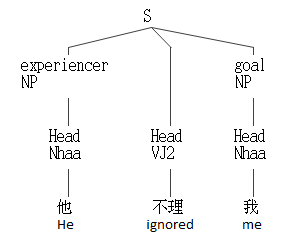
\includegraphics[width=.4\textwidth,height=3.9cm]{./examples/example5-english-subs.png}
\caption{An example tree from Sinica Treebank}
\end{figure}
\subsection{E-HowNet}
E-HowNet \cite{Chen:2010:EAC:1944284.1944296} is a semantic lexical knowledge-base for Chinese. It is a frame based entity-relation model that defines relationships between 2600 well-defined primitive concepts ("entities"). Around 90,000 Chinese words are categorized into different groups based on their sense similarity, and then those groups are tagged with the primitive concept they represent. For example, the entry 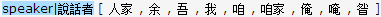
\includegraphics[width=.4\textwidth]{./examples/ehownet-snapshot.png} from E-HowNet shows that the nine Chinese words (enclosed in square brackets) share the same sense, and they belong to the primitive concept 'speaker'.

In this study, we use this grouping to generalize lexical statistics, and hence, to abate the effects of data sparseness on SRL. Throughout this paper, we have used the term "semantic type (\verb+semType+)" to refer to the primitive concept a given Chinese word represent. 
\section{Previous SRL System and Issues}
A semantic role labeling (SRL) system for Chinese was reported by \cite{you-chen:2004}. In that system, Sinica Treebank was used to train probabilistic models, which, together with a back-off strategy, were used for semantic role classification. As far feature set, the system relied on a number of conventional lexical features: target word (\verb+t+), target word pos (\verb+t_pos+), head word (\verb+h+), head word pos (\verb+h_pos+), and syntactic features: phrase type (\verb+pt+) and \verb+position+ (i.e. position of the target word with respect to the head word). The overall accuracy of the system was reported to be 92.71\%. Even though this accuracy can be considered on the higher side, there was room for improvement, especially in two subtasks: data sparseness handling and classification approach.

Data sparseness handling first, the previous system used a back-off strategy to tackle this problem -- see \cite{you-chen:2004} for more details. This considerably improved the baseline performance, but data sparseness still remained an issue. A major reason for this was dependency of the system on non-generalized lexical features (e.g. \verb+h_word+, \verb+t_word+). As mentioned previously, in the proposed system, we use E-HowNet to address this problem ( Section 5).

Classification methodology next. In the existing system, six probabilistic models, together with a back-off strategy, were used for semantic role assignment. As shown below, a particular feature combination was used for each model, and the backing-off was based on number of examples seen in the training data.
\begin{verbatim}
if#of(h,h_pos,t,t_pos,pt,position)
>threshold
P(r|constituent)=
P(r|h,h_pos,t,t_pos,pt,position)
else
if#of(h_pos,t,t_pos,pt,position)
>threshold
P(r|constituent)=
P(r|h_pos,t,t_pos,pt,position)
else
......
\end{verbatim}
A critical observation is that backing-off based on a constant threshold value does not allow to exploit the statistical knowledge in the best possible way. The reason is that if enough examples, with a more constrained feature combination, have been seen in the training data, the less constrained statistical information becomes irrelevant, which actually may suggest a more probable role. We propose a different strategy that is based on a combination of weighted probabilistic models. It utilizes the statistical knowledge in a better way, and hence, provide improvement in performance (see Section 4.3 for more details).
\section{Proposed SRL System}
The proposed SRL system is statistical. Its feature set, probabilistic models, and classification approach are given in the following subsections.  
\subsection{Feature Set}
\textbf{Lexical Features:} Part of speech tag of the target word (\verb+t_pos+), part of speech tag of the head word (\verb+h_pos+), part of speech tags of the immediate left and right siblings of a test node (\verb+l_r_ch_pos+),  a set of part of speech tags of all nodes under a test node including the test node itself (\verb+all_pos+).\\[0.2cm]
\textbf{Syntactic Features:} phrase type (\verb+pt+), a sentence-level boolean feature indicating weather the sentence containing the test node is passive or not (\verb+passive+), position of the target node w.r.t phrasal head (\verb+position+).\\[0.2cm]
\textbf{Semantic Features:} Semantic type of the head word extracted from E-HowNet (\verb+h_w_semType+), semantic type of the target word (\verb+t_w_semType+), a set of semantic types of all nodes of the tree the test node is a child of (\verb+all_semType+). \\[0.2cm]
Table 1 shows the values of these features for each constituent of the parse tree shown in Figure 1.
\begin{table}[!h]
\small
\begin{center}
\begin{tabular}{|p{2cm}|p{2cm}|p{2cm}|}
\hline \textbf{Semantic Role} & experiencer & goal \\ \hline
 \verb+t_w_semType+ & 3rdPerson  & speaker \\
 \verb+t_pos+ & NP &  NP \\ 
 \verb+h_w_semType+ &  ShowInterest & ShowInterest \\ 
 \verb+h_pos+ & VJ2 & VJ2 \\ 
 \verb+pt+ & S & S \\ 
 \verb+position+ & before & after \\ 
 \verb+passive+ & false & false \\ 
 \verb+l_r_ch_pos+ & empty-VJ2 & VJ2-empty\\ 
 \verb+all_pos+ & NP-Nhaa  & NP-Nhaa\\ 
 \verb+all_semType+ & 3rdPerson-ShowInterest-speaker  &  3rdPerson-ShowInterest-speaker\\ 
\hline 
\end{tabular}
\caption{Features-values of each constituent of Figure 1 parse tree.}
\end{center}
\normalsize 
\end{table}
\subsection{Probabilistic Models}
Ten probabilistic models were built using the Sinica Treebank labeled data. The probabilities were estimated using the following formula:
\begin{Verbatim}[commandchars=\\\{\},codes={\catcode`$=3\catcode`_=8}]
  $P(r|constituent)$  
   $= P(r|f_{c})$
   $= #(r,f_{c})/#f_{c}$
\end{Verbatim} 
Where $f_c$ represents a particular feature combination. A number of combinations were tested, and for the final system we used the set of ten combinations given in Table 2.
\begin{table}[!h]
\small
\begin{center}
\begin{tabular}{|c|p{6cm}|}
\hline \textbf{\#} & \textbf{Feature Combination} \\ 
\hline 1 & \verb+semType_h_w+, \verb+h_pos+, \verb+semType_t_w+, \verb+t_pos+, \verb+pt+, \verb+position+, \verb+all_pos+, \verb+passive+, \verb+all_semType+, \verb+l_r_ch_pos+ \\ 
 2 & \verb+h_pos+, \verb+t_w_semType+, \verb+t_pos+, \verb+pt+, \verb+position+, \verb+passive+\\ 
 3 & \verb+semType_h_w+, \verb+h_pos+, \verb+t_pos+, \verb+pt+, \verb+position+, \verb+passive+\\  
 4 &  \verb+semType_t_w+, \verb+t_pos+, \verb+pt+, \verb+position+, \verb+passive+\\   
 5 &  \verb+semType_h_w+, \verb+semType_t_w+, \verb+pt+, \verb+position+, \verb+passive+\\ 
 6 &  \verb+semType_t_word+, \verb+t_pos+, \verb+pt+, \verb+passive+\\ 
 7 &  \verb+semType_t_word+, \verb+t_pos+, \verb+pt+, \verb+passive+ \\ 
 8 &  \verb+semType_t_word+, \verb+t_pos+, \verb+passive+ \\ 
 9 & \verb+t_pos+, \verb+pt+, \verb+position+, \verb+passive+ \\ 
 10  & \verb+semType_t_w+ \\ 
\hline 
\end{tabular} %\begin{verbatim}
\caption{The set of feature combinations}
\normalsize
\end{center}
\end{table}
\subsection{Classification Method}
\subsubsection*{Notations}
\begin{itemize}
\item Let $F$ be the set of ten feature combinations (given in Table 2), and $f_c$ be an element of $F$
\item $P$ be the set of ten corresponding probabilistic models, and ${P_f}_c$ be an element of $P$ that is based on feature combination $f_c$ 
\item ${D_f}_c$ be the probability distribution computed by ${P_f}_c$ 
\item $M_{((p,r)|f_c)}$ be the $(probability,role)$ pair in  ${D_f}_c$ with highest probability
\item $W$ be a set of optimal weights, $w$ be an element of $W$, and $wp$ be a weighted probability (i.e. rank)
\end{itemize} 
\subsubsection*{Algorithm}
The proposed classification algorithm is:
\begin{enumerate}
\item For a test candidate, extract values of all features (mentioned in section 4.1) using the parse tree and E-HowNet.
\item initialize $potential\_roles$  $\leftarrow$ $empty$ 
\item For each $f_c$  $\in$ $F$ do:
\begin{itemize}
 \item Find probability distribution ${D_f}_c$ using the corresponding ${P_f}_c$ model
 \item Select $M_{((p,r)|f_c)}$ from ${D_f}_c$
 \item Rank $M_{((p,r)|f_c)}$ by multiplying $p$ with the corresponding $w$ from $W$
 \item Append $(wp,r)$ to $potential\_roles$
 \end{itemize}
\item Return the top ranked $r$ from $potential\_roles$
 \end{enumerate}
The major idea is to utilize both more and less constrained statistical knowledge in determining the semantic role. For this purpose ten probabilistic models are built. Each model is based on particular feature constraints, which are relaxed as we move from feature combination 1 to 10 in Table 2. The output of each model is ranked by learned weights, and the top ranked role is finally assigned to each test constituent. The weights, which encode the worth of a particular feature combination in determining the role, are learned using genetic algorithms and a held out development data set. The learned set of optimal weights is: % in order from \verb+w1+ to \verb+w10+ is: \verb+[0.9,1.0,0.9,0.7,0.8,0.4,0.5,0.4]+.
\begin{verbatim}
{(w1:0.9),(w2:1.0),(w3:0.9),
(w4:0.7),(w5:0.8),(w6:0.4),
(w7:0.5),(w8:0.4),(w9:0.5),
(w10:0.4)}
\end{verbatim} 
\section{Data Sparseness Handling}
As pointed by \cite{Gildea:2002}, lexical statistics, though very useful for semantic role labeling, often becomes a source of data sparseness. For the same reason, we replaced two lexical features (i.e. \verb+h_word+, and \verb+t_word+) used by the previous system with more general features (i.e. \verb+semType_h_word+ and \verb+semType_t_word+) respectively. Table 3 gives coverage and the corresponding accuracy statistics before and after adding these generalizations for each of the ten probabilistic models (given in Section 4.2). As can be seen, after generalization, the coverage improved considerably for each feature combination, which ultimately resulted in better performance.
\begin{table}[!h]
\small
\begin{center}
\begin{tabular}{|l|l|l|l|l|}
\hline
\multirow{2}{*}{\bf${P_f}_c$} & \multicolumn{2}{|l}{{\bf With Words}} & \multicolumn{2}{|l|}{\bf With Semantic Types} \\ \cline{2-5} 
                  &   Coverage       &      Accuracy     &     Coverage       &     Accuracy      \\ \hline
   1              &    7.10\%       &    23.61\%       &   12.68\%         &        28.00\%   \\ 
   2              &    52.06\%      &     59.14\%      &   73.05\%         &        74.98\% \\ 
   3              &    67.43\%      &     69.87\%      &   82.68\%         &        81.15\%   \\ 
   4              &    74.56\%       &     68.92\%     &   93.35\%          &        79.16\%  \\ 
   5              &    97.97\%      &      92.25\%     &   97.97\%         &         92.27\%  \\ 
   6              &    28.60\%       &     40.13\%      &  64.20\%          &        62.95\%   \\ 
   7              &    76.30\%       &     68.07\%      &  94.23\%          &        76.87\%  \\ 
   8              &    82.97\%       &      63.50\%     &  96.85\%          &        67.40\%  \\ 
   9              &    99.78\%       &      79.17\%     &   99.78\%         &        79.41\%   \\ 
   10             &    90.09\%       &      58.18\%     &   99.00\%         &          53.31\% \\ \hline
\end{tabular}  
\caption{Coverage \& Accuracy Statistics}
\end{center}
\label{tab:coverage-stats}
\end{table}
\normalsize
\section{Experiments and Evaluation}
To evaluate the performance and to show the usefulness of our approach, we built five semantic role labeling systems: (1) \textbf{DT:} Based on Decision Tree classifier, (2) \textbf{NB:} Based on Naive Bays classifier, (3) \textbf{ME:} Based on Maximum Entropy classifier, (4) \textbf{LI:} Based on probabilistic models together with linear interpolation, and (5) \textbf{WPM:} Based on the proposed weighted probabilistic models (WPM) classification approach. All of these systems were tested using the same feature set (given in Section 4.1), and the same training and testing data (i.e. Sinica Treebank). Results of a 10-fold cross validation scheme are given in Table 4. 
\begin{table}[!h]
\small
\begin{center}
\begin{tabular}{|l|c|c|}
\hline \bf System & \bf Accuracy &  \bf Precision\\ \hline
 DT & 91.03\% & 91.04\%  \\ 
 NB & 92.58\% & 92.57\% \\ 
 ME & 92.67\% & 92.68\% \\ 
 LI & 94.26\% &  94.27\%\\ 
 WPM & 94.49\% & 94.49\% \\ 
\hline 
\end{tabular}
\caption{Evaluation results} 
\end{center}
\normalsize
\end{table}
From the resulting numbers, we can see that our system outperformed all other systems.

To further enhance the performance of our system, we added a post-processing component to fix some of the obvious mistakes made by the probabilistic models. One such case is disambiguation between possessor/property roles. We used a heuristic rule that if the semantic type of a target word is \verb+human+, it is more likely to be a \verb+possessor+ than a \verb+property+. With few other such rules, the scores were improved from 94.49\% to 94.73\%. 
\section{Conclusion and Future Work}
In the scenario, where improving the performance of a SRL system by better engineering the feature-set looks more challenging, we have proposed an alternative way to achieve the same goal. We have presented a distinct classification approach, and the use of semantic knowledge to enhance the performance of an already reported SRL system. In conclusion, the proposed system outperformed a number of other systems, which were based on well-known classification approaches. With its better performance, the overall accuracy of the existing SRL system was improved from 92.71\% to 94.73\%. 

Since the proposed approach is language independent, in future, we have plans to experiment using the English and Chinese prop-bank data. Our hope is that we can improve state-of-the-art SRL scores.         
\clearpage
\bibliographystyle{acl}
\bibliography{eacl2014}

\end{document}
